%% 
%% Copyright 2019-2024 Elsevier Ltd
%% 
%% Version 2.4
%% 
%% This file is part of the 'CAS Bundle'.
%% --------------------------------------
%% 
%% It may be distributed under the conditions of the LaTeX Project Public
%% License, either version 1.2 of this license or (at your option) any
%% later version.  The latest version of this license is in
%%    http://www.latex-project.org/lppl.txt
%% and version 1.2 or later is part of all distributions of LaTeX
%% version 1999/12/01 or later.
%% 
%% The list of all files belonging to the 'CAS Bundle' is
%% given in the file `manifest.txt'.
%% 
%% Template article for cas-sc documentclass for 
%% single column output.

%\documentclass[a4paper,fleqn,longmktitle]{cas-sc}
\documentclass[a4paper,fleqn]{cas-sc}

%\usepackage[numbers]{natbib}
%\usepackage[authoryear]{natbib}
\usepackage[authoryear]{natbib}
\usepackage[utf8]{inputenc}
\usepackage[T1]{fontenc}    % Fixed hidden spaces here
\usepackage{hyperref}       % Fixed hidden spaces here
\usepackage{url}
\usepackage{booktabs}
\usepackage{amsfonts}
\usepackage{nicefrac}
\usepackage{microtype}
\usepackage{lipsum}
\usepackage{graphicx}
\usepackage{natbib}
\usepackage{doi}
\usepackage{tabularx}
\usepackage{multirow}
\usepackage{diagbox}
\usepackage{array}          % ADDED: Required for your table alignments
\usepackage{amsmath}
\usepackage{cleveref}       %
\usepackage{algorithm}
\usepackage{algorithmic}
\usepackage{booktabs}
\usepackage{placeins}
\usepackage{float}
\usepackage{xcolor}
\newcommand{\rev}[1]{\textcolor{red}{#1}}

\hypersetup{
    colorlinks=true,
    citecolor=blue,
    linkcolor=blue,
    urlcolor=blue
}
%%%Author macros
\def\tsc#1{\csdef{#1}{\textsc{\lowercase{#1}}\xspace}}
\tsc{WGM}
\tsc{QE}
\tsc{EP}
\tsc{PMS}
\tsc{BEC}
\tsc{DE}
%%%

\begin{document}
\let\WriteBookmarks\relax
\def\floatpagepagefraction{1}
\def\textpagefraction{.001}
% \shorttitle{Leveraging social media news}
% \shortauthors{J.K. Krishnan et~al.}
%\begin{frontmatter}

\title [mode = title]{Diverse Initializations for Vector Ensembles in Representation-aware Text-Attributed Graph Encoding with Large Language Models}   
\shorttitle{Diverse Initializations for Vector Ensembles in Representation-aware TAG Encoding with LLMs}                   
% \tnotemark[1,2]

% \tnotetext[1]{This document is the results of the research
%    project funded by the National Science Foundation.}

% \tnotetext[2]{The second title footnote which is a longer text matter
%    to fill through the whole text width and overflow into
%    another line in the footnotes area of the first page.}




% \cormark[2]
% \fnmark[1,3]
% \ead{t.rafeeq@example.in}
% \ead[URL]{www.campus.in}

% \cortext[cor1]{Corresponding author}
% \cortext[cor2]{Principal corresponding author}
% \fntext[fn1]{This is the first author footnote, but is common to third
%   author as well.}
% \fntext[fn2]{Another author footnote, this is a very long footnote and
%   it should be a really long footnote. But this footnote is not yet
%   sufficiently long enough to make two lines of footnote text.}

% \nonumnote{This note has no numbers. In this work we demonstrate $a_b$
%   the formation Y\_1 of a new type of polariton on the interface
%   between a cuprous oxide slab and a polystyrene micro-sphere placed
%   on the slab.
%   }

\begin{abstract}
Learning on text-attributed graphs requires combining rich node text with graph structure, but existing LLM--GNN methods often depend on expensive textual augmentation, external APIs, or a single fine-tuned encoder whose representations may be brittle for downstream graph learning.
This study addresses how to obtain diverse, high-quality text-derived node representations and combine them effectively for node classification without augmenting node text. We introduce DIVERGE, which repeatedly fine-tunes one LLM on native node texts and labels using diverse LoRA initializations, trains a GNN on each resulting embedding set, and adaptively ensembles the GNN pool with trainable model- and class-level weights.
On Cora, CiteSeer, PubMed, WikiCS, and OGBN-ArXiv, DIVERGE consistently outperformed classical GNNs and hybrid LLM--GNN baselines, reaching the best reported accuracy and Macro-F1 on all five benchmarks. Different initializations produced complementary embeddings, and learned ensembling outperformed uniform averaging. These findings show that representation diversity induced from native graph text can match or exceed augmentation-based approaches while reducing computational and API cost. Because all encoding runs on locally fine-tuned models without transmitting node text to third-party services, DIVERGE is also well suited to privacy-sensitive settings such as institutional repositories, enterprise document networks, and regulated biomedical corpora.
\end{abstract}

% \begin{graphicalabstract}
% \includegraphics{figs/cas-grabs.pdf}
% \end{graphicalabstract}

% \begin{highlights}
% \item Research highlights item 1
% \item Research highlights item 2
% \item Research highlights item 3
% \end{highlights}

\begin{keywords}
Text-Attributed Graphs \sep
Large Language Models \sep
Graph Neural Networks \sep
Ensemble Learning \sep
LLM on Graph \sep
Parameter-efficient fine-tuning \sep
Data privacy

\end{keywords}


\maketitle

\section{Introduction}

\textbf{Text-attributed graphs (TAGs)} model entities and their relationships through both network structure and associated text, appearing in social networks, citation graphs, and e-commerce platforms \citep{zhang2025leveraging, he2024harnessing}. \textbf{Graph neural networks (GNNs)} have traditionally processed these graphs using shallow embeddings or fine-tuned language models such as BERT \citep{devlin2018bert}. However, such encoders often fail to capture the semantic depth and world knowledge required for accurate node classification \citep{he2024harnessing, zhang2025leveraging}.

\textbf{Large language models (LLMs)}, including GPT and LLaMA, offer stronger contextual understanding and have motivated a new generation of LLM--GNN methods \citep{brown2020language, touvron2023llama}. Integrating LLMs with graphs nevertheless remains challenging because API-based annotation scales poorly to millions of nodes, exposes proprietary or sensitive node text to third-party cloud providers, and because LLM-generated features can introduce noise, hallucinations, and inference-time distribution shift \citep{Jaiswal2024AllAgainstSome, hu2025gaga, zhang2025leveraging}.


Recent research studies have addressed these hurdles through several innovative strategies:
\begin{itemize}
    \item \textbf{Explanations as Features:} Approaches such as \textbf{TAPE} leverage the reasoning abilities of LLMs by using their decision-making explanations as vectorial node features, which significantly boosts GNN performance without requiring full LLM fine-tuning  \citep{he2024harnessing}.
    \item \textbf{Efficient Integration and Inference:} Frameworks like \textbf{E-LLaGNN} utilize LLMs as an on-demand service to enhance only a tactical fraction of nodes, thereby reducing the computational footprint and facilitating \textbf{LLM-free inference} for industrial deployment  \citep{Jaiswal2024AllAgainstSome}.
    \item \textbf{Topological Structure Refinement:} Models like \textbf{GraphEdit} and \textbf{GAGA} employ LLMs to learn complex node relationships globally, effectively denoising connections by removing unreliable edges and adding reliable ones based on semantic similarity  \citep{guo2024graphedit, li2024gaga, Sun2026TopologicalEnhancerTAG}.
    \item \textbf{Cost-Effective Labeling:} New active self-training frameworks, such as \textbf{Locle}, identify "critical" samples for LLM annotation while utilizing GNN-based graph rewiring to refine labels, achieving state-of-the-art results for \textbf{label-free node classification} at a minimal cost  \citep{zhang2025leveraging}.
\end{itemize}

Despite this progress, three limitations motivate our work. First, augmentation-heavy pipelines such as TAPE \citep{he2024harnessing} depend on external LLM APIs and can hurt accuracy when node texts are already informative (Section~\ref{sec:Preliminaries}). Second, sending full node corpora to remote APIs creates privacy, retention, and compliance risks in institutional, enterprise, and regulated domains where graph text must remain on premises. Third, existing ensemble variants typically average GNN logits uniformly, which cannot exploit class-specific strengths of different representations. We therefore propose \textbf{DIVERGE}, a framework that induces diverse semantic views through multiple LoRA initializations and combines the resulting GNNs with adaptive, trainable weighting---without textual augmentation, paid API calls, or off-site disclosure of node text.


From an \textbf{information-processing perspective}, TAG node classification supports core tasks in bibliometrics, digital libraries, knowledge-base curation, knowledge graph and recommendation over linked documents \citep{Zhang2024TAGSurvey, RAMIREZMOLINA2026104842, WANG2026DGRLS}. Citation and hyperlink graphs encode how scientific ideas, web pages, and catalogued entities relate to one another; accurate categorization of nodes directly affects literature discovery, expert finding, and knowledge-network maintenance.

Our main contributions are as follows:
\begin{itemize}
	\item We propose \textbf{DIVERGE}, a novel framework for text-attributed graph learning that generates diverse semantic representations using multiple parameter-efficient LLM fine-tuning processes with different LoRA initialization strategies, without requiring textual augmentation or external LLM API calls.
	
	\item We introduce an adaptive ensemble learning framework that combines multiple GNNs trained on heterogeneous textual representations using trainable weighting mechanisms, including model-level and class-level aggregation strategies.
	
	\item We demonstrate that diverse representations can be effectively induced solely from the original graph texts and graph structure, eliminating the need for costly LLM-generated augmented texts while reducing computational and financial overhead and keeping all node text within the operator's trusted infrastructure---an important requirement for privacy-sensitive and compliance-constrained deployments.
\item We highlight a practical advantage of local, API-free encoding: DIVERGE never transmits proprietary node descriptions to external LLM services, which supports on-premises deployment in bibliographic systems, enterprise knowledge graphs, and regulated biomedical corpora where data residency and confidentiality constraints prohibit cloud-based augmentation.
	
	\item Extensive experiments on benchmark datasets, including Cora, CiteSeer, PubMed, WikiCS, and OGBN-ArXiv, show that the proposed method consistently outperforms existing GNN and hybrid LLM-GNN baselines across Accuracy and Macro-F1 metrics.
	
	\item Through ablation studies and statistical analysis, we show that different LoRA initialization strategies produce complementary semantic representations and that trainable ensemble learning significantly improves classification performance compared to simple averaging methods.
\end{itemize}

The structure of the paper is as follows: in Section~\ref{sec:relatedWork}, we review existing studies on integrating LLMs and GNNs for text-attributed graphs. Section~\ref{sec:Preliminaries} presents the motivation and preliminaries of the proposed framework. In Section~\ref{sec:Methodology}, the proposed DIVERGE methodology is described in detail, including the diverse LoRA initialization strategies, representation extraction process, and adaptive ensemble learning mechanisms. Section~\ref{sec:Evaluation} introduces the datasets, baselines, implementation details, and evaluation metrics used in the experiments. Section~\ref{sec:Results} reports the experimental results and ablation studies. Section~\ref{sec:Discussion} interprets these findings, articulates their theoretical and practical implications, and positions DIVERGE relative to prior work. Section~\ref{sec:Limitations} discusses the limitations of the proposed approach, and Section~\ref{sec:Conclusion} concludes the paper and outlines directions for future work.


\section{Research Objectives}\label{sec:researchObjectives}
Motivated by the limitations of augmentation-heavy LLM--GNN pipelines, this study addresses the following objectives:
\begin{enumerate}
    \item To induce diverse, complementary node representations from native graph texts using multiple LoRA initialization strategies, without textual augmentation, paid LLM APIs, or off-site exposure of sensitive node text.
    \item To design adaptive ensemble mechanisms that weight heterogeneous GNN outputs at model and class levels.
    \item To evaluate DIVERGE against GNN, encoder-, enhancer-, and predictor-based LLM--GNN baselines on five TAG benchmarks.
    \item To analyze when diversity-driven encoding outperforms augmentation-based approaches and quantify gains statistically.
\end{enumerate}

\section{Related Works}\label{sec:relatedWork}
LLMs have recently been integrated with GNNs for processing TAGs. Based on existing studies, We categorize the role of LLMs into three main paradigms: Encoder, Enhancer, and Predictor \citep{Wu2025LLMNode, Jin2023LLMGraphs, Chen2024LLMGraphs, Li2024GraphLLMSurvey}.

\subsection{LLMs as Encoders}
The \textbf{Encoder} paradigm uses LLMs to map node text to vector representations that downstream GNNs consume \citep{he2024harnessing, Huang2024GNNAdapters, Zhu2024EfficientTextualGraphs}. Early pipelines relied on shallow features (bag-of-words, skip-gram); recent methods employ pre-trained LMs or LLMs as text encoders. \textbf{ENGINE} \citep{Zhu2024EfficientTextualGraphs} optimizes end-to-end efficiency for large TAGs through parameter-efficient LLM tuning. \textbf{GraphAdapter} \citep{Huang2024GNNAdapters} injects structural signals into frozen LLMs via lightweight adapters \citep{Houlsby2019Adapters}. \textbf{WalkLM} \citep{Tan2023WalkLM} textualizes random walks to joint learning of text and topology, while \textbf{One-for-All (OFA)} \citep{liu2024oneforall} seeks a unified semantic space across graph domains. \textbf{LEADING} \citep{Xue2025LEADING} further reduces label demand through neighbor decoupling during end-to-end LM--GNN training. \textbf{STAGE} \citep{zolnai-lucas-etal-2024-stage} demonstrates that frozen LLM embeddings combined with ensemble GNN training can be competitive on academic TAGs with minimal pipeline complexity.

\citet{Wu2025LLMNode} release \textbf{LLMNodeBed} and systematically ask \emph{when} LLMs help node classification. Their analysis shows that (a)~encoder-style LLM features consistently outperform bag-of-words and shallow LM baselines on most TAG benchmarks, (b)~enhancement-heavy pipelines do not always justify their cost, and (c)~predictor-style LLM methods are sensitive to prompting and scale. These findings motivate DIVERGE's focus on strong \emph{local} encoders rather than paid API augmentation.\textbf{LLM-BP} \citep{wang2025llmbp} proposes task-adaptive LLM embeddings and belief-propagation-style aggregation, improving cross-graph generalization on 11 TAG datasets. DIVERGE differs from LLM-BP by inducing diversity through multiple LoRA initializations of a \emph{single} backbone rather than task-adaptive prompting, and by learning ensemble weights over GNN logits rather than propagating beliefs on a single embedding space.

\subsection{LLMs as Enhancers}
Enhancer methods modify node text, graph structure, or labels before or during GNN training. \textbf{TAPE} \citep{he2024harnessing} generates LLM explanations and zero-shot predictions to enrich node text, then trains multiple GNNs whose logits are \emph{uniformly averaged}. Although effective on several benchmarks, TAPE requires external LLM API access and can introduce semantic noise when native texts are already informative (Section~\ref{sec:Preliminaries}). Structural enhancers include \textbf{RoSE} \citep{Sun2026TopologicalEnhancerTAG} and \textbf{GraphEdit} \citep{guo2024graphedit}. \textbf{LLM4NG} \citep{Yu2025NodeGenerationTAG} synthesizes nodes and edges for few-shot TAG learning.

A second enhancer thread targets \textbf{cost and label efficiency}. \textbf{E-LLaGNN} \citep{Jaiswal2024AllAgainstSome} enhances only critical nodes to enable LLM-free inference at deployment. \textbf{Locle} \citep{zhang2025leveraging} combines active LLM labeling with GNN-based graph rewiring for label-scarce node classification. \textbf{GAGA} \citep{hu2025gaga} annotates representative nodes and aligns an annotation graph with the TAG, requiring as little as 1\% labeled data in reported experiments. \textbf{UltraTAG} \citep{yu2025ultratag} modularizes augmentation, text encoding, and training into a unified robust pipeline (with extensions such as UltraTAG-S for sparse text/edges). \textbf{SKETCH} \citep{zhou-etal-2025sketch} decouples semantic and structural aggregation: it retrieves related node texts and distant structural contexts before long-context LM training, reducing reliance on conventional GNN propagation while improving efficiency.

Collectively, enhancer methods demonstrate that LLMs can improve TAG learning by enriching inputs---but often at the cost of API fees, hallucination risk, or complex multi-stage pipelines. DIVERGE deliberately avoids textual augmentation and instead asks whether comparable gains can arise from \emph{diverse encodings of native text}.

\subsection{LLMs as Predictor}
In the \textbf{Predictor} paradigm, LLMs directly perform reasoning tasks on text-attributed graphs. Methods like \textbf{GRAPHTEXT} transform graph structures into "Graph-Syntax Trees" that are flattened into textual sequences, allowing LLMs to reason over the graph as a text-generation task \citep{Zhao2024GraphText}. Other approaches adapt LLMs to better capture structural knowledge by mapping graphs into ordered node sequences or injecting structural embeddings into the LLM's input space using projectors or prefix tuning, as seen in \textbf{DGTL} \citep{Qin2024DisentangledTAG} and \textbf{LLaGA} \citet{Chen2024LLaGA}. Additionally, the \textbf{ZeroG} framework explores cross-dataset zero-shot transferability, leveraging a shared semantic space to apply graph knowledge without task-specific fine-tuning \citep{Li2024ZeroG}.These methods lie outside our encoder–GNN
design and are included only as baselines in Section \ref{sec:Evaluation}.

\subsection{Ensemble learning and representation diversity}

Ensembling multiple graph learners is not new, but \emph{how} models are combined varies widely. TAPE averages GNN logits with fixed equal weights \citep{he2024harnessing}. STAGE and LLMNodeBed benchmarks show that even simple encoder ensembles can be strong \citep{zolnai-lucas-etal-2024-stage, Wu2025LLMNode}. LLM-BP advances aggregation through learned, graph-adaptive belief propagation \citep{wang2025llmbp}. Yet most LLM--GNN pipelines still derive diversity from \emph{different modalities or pipeline stages} (e.g., augmented vs.\ original text, LM vs.\ GNN), not from multiple parameter-efficient trajectories of the same encoder.

In parallel, parameter-efficient fine-tuning (PEFT) research shows that initialization and low-rank adaptation strategy affect the semantic subspace an LM converges to \citep{Hu2021LoRA, meng2024pissa, paischer2024eva, li2023loftq, zhang2025orthogonal, wang2025peft}. DIVERGE extends this insight to TAGs: we treat \textbf{LoRA initialization diversity} as a controllable source of complementary node representations and combine the resulting GNNs with \textbf{learned} model- and class-level weights rather than uniform averaging.

\subsection{Research gap and position of DIVERGE}

\begin{table}[htbp]
\centering
\caption{Comparison of DIVERGE with representative recent TAG methods (2024--2025).}
\label{tab:related_gap}
\small
\begin{tabular*}{\linewidth}{@{\extracolsep{\fill}} lcccc @{}}
\toprule
\textbf{Method} & \textbf{Augment.\ text?} & \textbf{External API?} & \textbf{Diversity source} & \textbf{Aggregation} \\
\midrule
TAPE \citep{he2024harnessing} & Yes & Yes & Multi-feature/GNN pool & Uniform average \\
UltraTAG \citep{yu2025ultratag} & Yes (module) & Optional & Pipeline modules & Task-specific \\
LLM-BP \citep{wang2025llmbp} & No & Optional & Task-adaptive encoder & Belief propagation \\
SKETCH \citep{zhou-etal-2025sketch} & No (retrieval) & No & Retrieved contexts & LM-centric \\
STAGE \citep{zolnai-lucas-etal-2024-stage} & No & No & Frozen LLM & Ensemble GNN \\
\textbf{DIVERGE (ours)} & \textbf{No} & \textbf{No} & \textbf{Multi-init LoRA} & \textbf{Learned ensemble} \\
\bottomrule
\end{tabular*}
\end{table}

Table~\ref{tab:related_gap} summarizes how DIVERGE relates to representative recent methods. No prior TAG approach simultaneously (1)~induces representation diversity through \textbf{multi-initialization LoRA} on native node text, (2)~trains a \textbf{pool of GNNs} on complementary embeddings, and (3)~fuses predictions with \textbf{learned ensemble weights}---all \textbf{without} LLM-based textual augmentation or external API calls. Methods such as TAPE and UltraTAG rely on augmentation; LLM-BP and SKETCH introduce diversity through task-adaptive prompting or retrieval;STAGE use a single encoding trajectory. DIVERGE fills this gap by showing that initialization-driven diversity plus adaptive ensembling can match or exceed augmentation-based performance (Section~\ref{sec:resultsAnalysis}) while remaining deployable in privacy-sensitive information systems (Section~\ref{sec:Discussion}).


\section{Preliminaries}\label{sec:Preliminaries}
\subsection{Motivation}

Recent studies on TAGs have shown that the quality and richness of node-associated texts play a critical role in the final performance of graph learning models \citep{he2024harnessing}. In citation networks and scientific document graphs, node texts often already contain highly informative semantic content that can strongly support downstream node classification tasks. Consequently, the effectiveness of graph representation learning increasingly depends on how efficiently this semantic information is extracted and utilized.

LLMs have recently emerged as powerful semantic encoders due to their strong contextual understanding and extensive linguistic knowledge. Several recent methods utilize LLMs to augment node texts by generating explanations, summaries, or pseudo-label descriptions for graph nodes \citep{he2024harnessing}. The underlying assumption of these approaches is that additional generated textual information can enrich node semantics and improve graph learning performance.



\begin{table}[h]
\caption{Accuracy of GNNs using different initial node features on the Cora dataset.}
\label{tab:gnn_features_comparison}

\begin{tabular*}{\linewidth}{@{\extracolsep{\fill}} lc @{}}
\toprule
\textbf{Type of Initial Node Features} & \textbf{Accuracy (\%)} \\
\midrule
Embeddings of original graph node texts & 89.14 \\
Embeddings of texts augmented by LLMs (zero-shot prediction) & 87.77 \\
Bag-of-words features & 85.34 \\
\bottomrule
\end{tabular*}
\end{table}

However, experimental observations reveal that textual augmentation is not always beneficial, particularly in graphs whose original node texts are already rich and informative. In such scenarios, generated texts may introduce semantic noise, hallucinated information, or incorrect predictions, which can ultimately degrade downstream graph performance. Table \ref{tab:gnn_features_comparison} demonstrates this phenomenon on the Cora dataset, where embeddings extracted directly from the original graph texts outperform embeddings derived from LLM-augmented texts.

Furthermore, augmentation-based methods impose substantial computational and financial costs. Many existing approaches rely on repeated calls to closed-source LLM APIs in order to generate augmented texts for all graph nodes. According to \citet{he2024harnessing}, the augmentation cost for a graph containing approximately 130 thousand nodes exceeded 125 US dollars. Such costs become increasingly prohibitive for large-scale graphs and real-world applications. Equally important, API-based augmentation requires uploading node texts---which may include unpublished manuscripts, internal reports, patient-related abstracts, or other confidential material---to third-party providers, raising data-residency, retention, and regulatory concerns. DIVERGE avoids this risk by fine-tuning and encoding entirely on local graph text.
These observations raise a more fundamental question: 
Can competitive or even superior performance be achieved without performing any textual augmentation, solely by making more effective use of the original graph texts and graph structure?

In this work, we hypothesize that representation diversity itself can serve as an alternative source of complementary information for text-attributed graph learning. Instead of generating additional texts, we investigate whether multiple semantic views can be extracted directly from the original node texts through different parameter-efficient fine-tuning trajectories of the same LLM.

Recent studies in optimization and representation learning suggest that different parameter initializations may guide neural networks toward different local minima, potentially producing complementary semantic representations. Motivated by this observation, we employ multiple LoRA fine-tuning processes using different initialization strategies. Although all models are trained on identical graph texts and labels, each initialization strategy can induce a distinct semantic interpretation of node texts, resulting in diverse node-level embeddings.

These diverse representations are subsequently used to train multiple independent GNNs. However, simply combining the outputs of these graph models through uniform averaging may not fully exploit the complementary strengths of different representations. In practice, some representations may perform better for specific classes or graph regions, while others may capture alternative semantic structures more effectively.

Therefore, this work additionally investigates adaptive ensemble learning strategies capable of learning the relative importance of different graph models. By assigning trainable weights at both the model and class levels, the proposed framework aims to more effectively combine complementary representations and improve overall graph learning performance.

Based on these motivations, we propose \textbf{DIVERGE}, a framework that integrates diverse parameter-efficient LLM fine-tuning with adaptive ensemble learning for robust and scalable learning on text-attributed graphs.




\subsection{Main Objective of the Proposed Method}
The main objective is to generate diverse representations of node texts (without augmenting or modifying the original node texts) and subsequently apply ensemble learning on GNNs trained using these representations.

Graphs with textual features are graphs in which each node is associated with a text (document). In this work, a graph with textual features is defined as follows:
\begin{equation}
G = (V, E, D, Y),
\end{equation}
where:
\begin{itemize}
\item $V=\{v_1,\dots,v_N\}$ is the set of nodes,
\item $E \subseteq V\times V$ is the set of edges,
\item $D=\{d_{v_1},\dots,d_{v_N}\}$ is the set of node texts, where $d_{v_i}$ is the text corresponding to node $v_i$,
\item $Y=\{y_1,\dots,y_N\}$ is the set of node labels, and
\item $y_i \in \{1,\dots,C\}$ denotes the label of node $v_i$ among $C$ classes.
\end{itemize}

Assume that a pre-trained LLM is available as a parametric function $\,f(\cdot;\mathbf{W})\,$. The input of this function is the node text, and its parameters correspond to the pre-trained weights:
\begin{equation}
f(x;\mathbf{W}), \qquad \mathbf{W}\in\mathbb{R}^{d\times k},
\end{equation}
where $x$ is the input text and $\mathbf{W}$ represents the model weights.

For fine-tuning the language model, the training set consisting of (text, label) pairs is defined as:
\begin{equation}
(D_{\text{train}},Y_{\text{train}})=\{(d_i,y_i)\}_{i\in\mathcal{I}_{\text{train}}}.
\end{equation}
The objective is to minimize the loss function over the training data:
\begin{equation}
\min_{\mathbf{W}} \ \mathcal{L}\big(f(x;\mathbf{W}), y\big).
\end{equation}

However, optimizing all parameters $\mathbf{W}$ (with dimensions $d\times k$) is computationally expensive; therefore, parameter-efficient fine-tuning methods are employed. In this work, the selected method is LoRA, which learns only a low-rank update instead of training all parameters:
\begin{equation}
\mathbf{W}'=\mathbf{W}+\Delta\mathbf{W}, \qquad \Delta\mathbf{W}=\mathbf{B}\mathbf{A},
\end{equation}
where:
\begin{equation}
\mathbf{B}\in\mathbb{R}^{d\times r}, \qquad \mathbf{A}\in\mathbb{R}^{r\times k}, \qquad r\ll \min(d,k).
\end{equation}

As a result, the optimization problem is reduced to training only the parameters $\mathbf{A},\mathbf{B}$:
\begin{equation}
\min_{\mathbf{A},\mathbf{B}} \ \mathcal{L}\big(f(x;\mathbf{W}+\mathbf{B}\mathbf{A}),y\big).
\end{equation}

After optimization, the resulting model is denoted by $\bar{f}$, which combines the original weights and the low-rank update:
\begin{equation}
\bar{f}(x)=f(x;\mathbf{W}+\mathbf{B}\mathbf{A}).
\end{equation}

For initializing the low-rank matrices, an initialization strategy is employed:
\begin{equation}
(\mathbf{A}^{(0)},\mathbf{B}^{(0)})\sim \mathcal{I}.
\end{equation}

\section{Methodology}\label{sec:Methodology}
\begin{algorithm}[t]
\caption{Proposed DIVERGE Framework}
\label{alg:framework}
\begin{algorithmic}

\REQUIRE Graph $G=(V,E,D,Y)$, pre-trained LLM $f$, number of LoRA runs $M$
\ENSURE Predicted node labels $\hat{Y}$

\FOR{$i=1$ to $M$}
    \STATE Initialize LoRA parameters with initialization $\mathcal{I}_i$
    \STATE Fine-tune LLM to obtain adapted model $\bar{f}_i$
    \STATE Extract node features $\mathbf{Z}^{(i)}$ from node texts using $\bar{f}_i$
    \STATE Train GNN on $(G,\mathbf{Z}^{(i)})$
    \STATE Obtain node logits $\mathbf{L}^{(i)}$
\ENDFOR

\STATE Collect logits $\bar{\mathbf{L}}=\{\mathbf{L}^{(i)}\}_{i=1}^{M}$
\STATE Train ensemble model on $\bar{\mathbf{L}}$
\STATE Aggregate logits and predict labels $\hat{Y}$

\RETURN $\hat{Y}$

\end{algorithmic}
\end{algorithm}
\begin{figure}
    \centering
    \includegraphics[width=1\textwidth]{images/diverge.png}
    \caption{Overview of a diverse fine-tuning and ensemble framework combining multiple LoRA-adapted LLMs models, GNN-based node representation learning, and adaptive MLP fusion for final node classification.
}
    \label{fig:diverge}
\end{figure}
\FloatBarrier
\subsection{Training LoRA Parameters of LLMs with Different Initializations}

To generate diverse representations, multiple LoRA fine-tuning runs with different initializations are performed. In other words, for each iteration $i$, an independent initialization strategy $\mathcal{I}_i$ is defined:
\begin{equation}
(\mathbf{A}^{(0)}_i,\mathbf{B}^{(0)}_i)\sim \mathcal{I}_i,\qquad i=1,\dots,M.
\end{equation}

Then, for each initialization, the language model is fine-tuned only through training the low-rank parameters:
\begin{equation}
\min_{\mathbf{A}_i,\mathbf{B}_i}\ \mathcal{L}\big(f(x;\mathbf{W}+\mathbf{B}_i\mathbf{A}_i),y\big).
\end{equation}

By solving the above optimization problem, the $i$-th fine-tuned model is obtained as:
\begin{equation}
\bar{f}_i(x)=f(x;\mathbf{W}+\mathbf{B}_i\mathbf{A}_i).
\label{eq:fbar}
\end{equation}

Finally, the collection of fine-tuned language models is defined as:
\begin{equation}
\mathcal{M}=\{\bar{f}_i\}_{i=1}^{M}.
\end{equation}

\subsection{Extracting Node-Level Feature Sets Using the Trained Models}

At this stage, the goal is to convert the text of each node into a node-level feature vector using the models
$\bar{f}_i$
(Equation \ref{eq:fbar}).

For node $v$, let the corresponding text be denoted by $d_v$, which after tokenization consists of $T$ tokens:
\begin{equation}
d_v=\{x_1,\dots,x_T\}.
\end{equation}

The output of the final layer of model $\bar{f}_i$ for the tokens is considered as a sequence of vectors:
\begin{equation}
\mathbf{H}^{(i)}_v=\big(\mathbf{h}^{(i)}_{1},\dots,\mathbf{h}^{(i)}_{T}\big), \qquad \mathbf{h}^{(i)}_{t}\in\mathbb{R}^{p},
\end{equation}
where $\mathbf{h}^{(i)}_{t}$ is the representation of token $t$ in the final layer.

To construct a node-level representation, mean pooling over tokens is used:
\begin{equation}
\mathbf{z}^{(i)}_{v}=\frac{1}{T}\sum_{t=1}^{T}\mathbf{h}^{(i)}_{t}.
\end{equation}

By stacking node vectors together, the node-level feature matrix for the $i$-th model is obtained:
\begin{equation}
\mathbf{Z}^{(i)}=\big[\mathbf{z}^{(i)}_{v_1},\dots,\mathbf{z}^{(i)}_{v_N}\big]^{\top}\in\mathbb{R}^{N\times p}.
\end{equation}

Consequently, the set of extracted features from all fine-tuned language models is:
\begin{equation}
\mathcal{F}=\{\mathbf{Z}^{(i)}\}_{i=1}^{M}.
\end{equation}

\subsection{Training Multiple GNNs Using the Extracted Features}

After obtaining the feature sets, a GNN is trained for each feature matrix $\mathbf{Z}^{(i)}$. The GNN is defined as a function $g(\cdot)$ operating on the graph and node features:
\begin{equation}
g_i = \mathrm{GNN}(G,\mathbf{Z}^{(i)}), \qquad i=1,\dots,M.
\end{equation}

For each node $v$, the output of network $g_i$ is a logit vector over the $C$ classes:
\begin{equation}
\boldsymbol{\ell}^{(i)}_{v}=\big(\ell^{(i)}_{v,1},\dots,\ell^{(i)}_{v,C}\big)\in\mathbb{R}^{C}.
\end{equation}

The logits of all nodes for the $i$-th model are summarized as:
\begin{equation}
\mathbf{L}^{(i)}=\{\boldsymbol{\ell}^{(i)}_{v_1},\dots,\boldsymbol{\ell}^{(i)}_{v_N}\}.
\end{equation}

Finally, the set of outputs (logits) from all GNNs is:
\begin{equation}
\bar{\mathbf{L}}=\{\mathbf{L}^{(i)}\}_{i=1}^{M}.
\end{equation}

\subsection{Training the Ensemble Learning Model}

At this stage, an ensemble learning framework is designed using the logits obtained from the $M$ GNNs. Unlike methods such as TAPE, which employ simple averaging of logits, the proposed method assumes that not all models contribute equally; therefore, adaptive weighting can improve the final performance.

The data used for training the ensemble learning model is defined as:
\begin{equation}
(\bar{\mathbf{L}}_{\text{train}}, y_{\text{train}}).
\end{equation}

\paragraph{Method 1: Model-Level Weighting}

In this method, each graph model is assigned a learnable weight in order to determine the relative importance of each model. The weight vector is defined as:
\begin{equation}
\boldsymbol{\theta}\in\mathbb{R}^{M}, \qquad \sum_{i=1}^{M}\theta_i=1,\ \ \theta_i\ge 0.
\end{equation}

These weights are learned using an MLP, and a softmax layer is applied at the output to satisfy the above constraints. The combined logits for node $v$ are computed as:
\begin{equation}
\bar{\boldsymbol{\ell}_{v}}=\sum_{i=1}^{M}\theta_i\,\boldsymbol{\ell}^{(i)}_{v}.
\end{equation}

The parameters of the ensemble model are trained by minimizing the loss:
\begin{equation}
\min_{\boldsymbol{\theta}}\ \mathcal{L}\big(\mathrm{MLP}(\bar{\mathbf{L}};\boldsymbol{\theta}),Y\big).
\end{equation}

\paragraph{Method 2: Class-Level Weighting}

In this method, an independent weight is assigned to each model and each class, allowing each model to contribute more strongly to the classes in which it performs better:
\begin{equation}
\mathbf{\Theta}\in\mathbb{R}^{M\times C}, \qquad
\sum_{i=1}^{M}\Theta_{i,c}=1,\ \ \Theta_{i,c}\ge 0 \ \ \forall c.
\end{equation}

The combined logits for node $v$ are computed as:
\begin{equation}
\bar{\ell_{v}}=\sum_{i=1}^{M}\Theta_{i,c}\ \ell^{(i)}_{v,c}.
\end{equation}

The parameters $\mathbf{\Theta}$ are also learned using an MLP with a softmax layer applied separately for each class.

\paragraph{Method 3: Class-Level Weighting with Independent Networks}

This method is similar to Method 2, with the difference that an independent MLP is defined for each class $c$. The goal of this design is to increase flexibility in learning complex and distinct weighting patterns across classes:

\begin{equation}
\mathbf{\Theta}_{:,c}=\mathrm{MLP}_c(\bar{\mathbf{L}}), \qquad c=1,\dots,C.
\end{equation}

\paragraph{Final Prediction}

After computing the aggregated logits for each node, the predicted label is determined using the argmax operation:

\begin{equation}
\hat{y}_v=\arg\max_{c\in\{1,\dots,C\}}\ \bar{\ell_{v,c}}.
\end{equation}

\section{Evaluation}\label{sec:Evaluation}
\subsection{Datasets}

\begin{table*}[t]
\caption{Specifications of the text-attributed graph benchmarks used in this study. Train/validation/test counts follow a random 60/20/20 split. Average degree is computed as $2|E|/|V|$ for undirected graphs.}
\label{tab:datasets}
\small
\begin{tabular*}{\textwidth}{@{\extracolsep{\fill}} lccccc @{}}
\toprule
\textbf{Statistic} & \textbf{Cora} & \textbf{CiteSeer} & \textbf{PubMed} & \textbf{OGBN-ArXiv} & \textbf{WikiCS} \\
\midrule
\textbf{Nodes} & 2,708 & 3,186 & 19,717 & 169,343 & 11,701 \\
\textbf{Edges} & 5,429 & 4,277 & 44,338 & 1,666,243 & 215,863 \\
\textbf{Classes} & 7 & 6 & 3 & 40 & 10 \\
\textbf{Train nodes} & 1,624 & 1,912  & 11,830 & 101,606  & 7,020 \\
\textbf{Validation nodes} & 541 & 637 & 3943 & 33869  & 2340 \\
\textbf{Test nodes} & 542 & 638  & 3944 & 33869  & 2341 \\
\textbf{Avg.\ tokens per node} & 82 & 72 & 79 & 63 & 629 \\
\textbf{Avg.\ degree} & 3.89 & 2.65 & 4.49 & 19.67 & 36.89 \\
\textbf{Node text} & Title + abstract & Title + abstract & Title + abstract & Title + abstract & Full article text \\
\textbf{Domain} & Machine learning & Computer science & Biomedical & Computer science & Computer science \\
\bottomrule
\end{tabular*}
\end{table*}

We evaluated DIVERGE on five widely used text-attributed graph (TAG) benchmarks obtained from the \textbf{LLMNodeBed} repository \citep{Wu2025,Wu2025LLMNode}, which provides standardized node texts, graph structures, and labels for fair comparison of LLM--GNN methods. The original dataset sources are Cora \citep{cora}, CiteSeer \citep{giles1998citeseer}, PubMed \citep{pubmed}, OGBN-ArXiv \citep{hu2020ogb}, and WikiCS \citep{mernyei2020wikics}. Table~\ref{tab:datasets} summarizes graph scale, textual properties, and split sizes; together, the five benchmarks comprise \textbf{206,655 nodes} and \textbf{1.94 million edges}.

\paragraph{Source and license.}
Cora, CiteSeer, and PubMed are classic citation-network benchmarks released for research use in the graph-learning literature \citep{cora,giles1998citeseer,pubmed}. OGBN-ArXiv is distributed under the Open Graph Benchmark (OGB) license \citep{hu2020ogb}. WikiCS is publicly available for non-commercial research \citep{mernyei2020wikics}. In our experiments, all graphs and node texts were accessed through the LLMNodeBed Hugging Face release \citep{Wu2025}, which harmonizes raw texts and graph topology across TAG baselines.

\paragraph{Node text content and label definition.}
Each node represents a document (or Wikipedia article) associated with a categorical label:
\begin{itemize}
    \item \textbf{Cora:} Each node is a machine-learning publication. Node text concatenates the paper \textbf{title and abstract} (mean 82 tokens). Labels denote one of seven research topics (e.g., neural networks, rule learning, reinforcement learning).
    \item \textbf{CiteSeer:} Each node is a computer-science publication with \textbf{title and abstract} text (mean 72 tokens). Labels indicate one of six paper categories.
    \item \textbf{PubMed:} Each node is a biomedical abstract related to diabetes. Node text consists of the \textbf{title and abstract} (mean 79 tokens). Labels indicate one of three disease categories (experimental induced diabetes, type~1 diabetes, type~2 diabetes).
    \item \textbf{OGBN-ArXiv:} Each node is a computer-science paper indexed in the arXiv MAG corpus. Node text combines \textbf{title and abstract} (mean 63 tokens). Labels correspond to one of 40 arXiv subject areas (e.g., cs.AI, cs.LG).
    \item \textbf{WikiCS:} Each node is a Wikipedia article from the computer-science subset. Node text is the \textbf{full article content} (mean 629 tokens), making it the most text-dense benchmark in our study. Labels denote one of ten Wikipedia category tags.
\end{itemize}
\paragraph{Graph construction.}
For Cora, CiteSeer, and PubMed, undirected edges represent mutual citation links between papers. For OGBN-ArXiv, directed citation links from the OGB release were treated as \textbf{undirected} edges to match standard GNN-based TAG protocols \citep{Wu2025LLMNode}. For WikiCS, undirected edges represent hyperlinks between Wikipedia pages. \textbf{Self-loops were not added} to the adjacency matrices; graph convolution used the standard neighbor aggregation of GraphSAGE on the provided topology.
\paragraph{Data splits.}
All experiments use a \textbf{random 60/20/20 split} for training, validation, and test nodes, with split sizes reported in Table~\ref{tab:datasets}. The split was performed once per dataset with a fixed random seed and held constant across all LoRA initializations, GNN models, and ensemble variants. Reported baseline results for classical GNNs and hybrid LLM--GNN methods are taken from \citet{Wu2025LLMNode}, which evaluates on the same LLMNodeBed benchmarks and split protocol; this ensures a like-for-like comparison. Where a baseline originally used a different split (e.g., the standard Planetoid per-class split), \citet{Wu2025LLMNode} re-evaluated it under the unified TAG setting.
\paragraph{Text preprocessing.}
Node texts were tokenized with the \textbf{Llama-3.2 tokenizer}. Sequences longer than \textbf{512 tokens} were truncated from the right; shorter sequences were padded during batching. Empty or missing texts were not present in the LLMNodeBed releases used here; if truncation removed tail content (notably on WikiCS), mean pooling was applied over all non-padding tokens of the final LLM hidden layer. Bag-of-words baselines in comparative tables used the preprocessed token statistics bundled with LLMNodeBed \citep{Wu2025LLMNode}.}
\paragraph{Class distribution and imbalance.}
Cora and CiteSeer are moderately balanced across classes (largest class $\approx$1.3--1.5$\times$ the smallest). PubMed is \textbf{imbalanced}: the majority class (type~2 diabetes) contains roughly twice as many nodes as the minority class (experimental induced diabetes). WikiCS exhibits mild imbalance across its ten categories. OGBN-ArXiv is the most challenging with \textbf{40 fine-grained labels} and moderate long-tail imbalance.
\paragraph{Summary.}
These benchmarks span citation and hyperlink graphs from machine learning, general computer science, biomedicine, and Wikipedia, with node counts from 2.7K to 169K and average degrees from 2.68 to 36.90. This diversity allows us to test whether representation diversity and adaptive ensembling generalize across graph scale, text length, domain, and label granularity.
\subsection{Baselines}
The baseline methods used for comparison with the proposed method are categorized into four general groups:
\begin{itemize}
    \item Classical GNN-based methods
    \item LLMs as Encoders
    \item LLMs as Enhancers
    \item LLMs as Predictors
\end{itemize}

In the first category, three well-known GNN methods were utilized: GCN  \citep{Kipf2016GCN}, GraphSAGE  \citep{hamilton2017sage}, and GAT  \citep{Velickovic2018GAT}. In these methods, textual features were converted into numerical vectors using the \textbf{Bag-of-Words} approach. In other words, \textbf{shallow embeddings} were used to represent the textual information of the nodes.

In the second category, serving as encoders and without fine-tuning, two language models—Sentence-BERT  \citep{reimers2019sentencebert} and RoBERTa  \citep{zhuang2021robustly}—were employed to transform textual features into richer vector representations. These representations were then provided as input to the GNNs, and the models were trained in a hybrid fashion. Additionally, the ENGINE  \citep{Zhu2024EfficientTextualGraphs} method was considered in the encoder role, which aims to achieve the best possible performance while optimizing training time and memory consumption.

In the third category, LLMs were examined as enhancers. To this end, the TAPE  \citep{he2024harnessing} method, which also inspired the proposed method, was used as one of the comparative baselines.

Finally, in the fourth category acting as predictors, two methods—GraphGPT  \citep{tang2024graphgpt} and LLaGA \citep{Chen2024LLaGA}—were reviewed, in which LLMs are used directly to perform the prediction task.

%The results for these methods have been extracted from the tables and charts presented by \citep{Wu2025LLMNode}.

\subsection{Experiments Settings and Implementation Details}
In the experiments conducted to transform text into semantic vector features, the \href{https://huggingface.co/meta-llama/Llama-3.2-1B}{LLaMA 3.2} model with one billion parameters was utilized. Additionally, the GraphSAGE model  \citep{hamilton2017sage} was employed for the implementation of the GNN. To fine-tune the models, the LoRA method  \citep{Hu2021LoRA} was applied.

\begin{table*}[t]
    \centering
    \caption{Main hyperparameters for DIVERGE training}
    \label{tab:hyperparams}
    \small
    \begin{tabular*}{\textwidth}{@{\extracolsep{\fill}} ll @{}}
    \toprule
    \textbf{Component} & \textbf{Setting} \\
    \midrule
    \multicolumn{2}{l}{\textit{Shared LLM / LoRA settings}} \\
    \midrule
    LLM backbone & LLaMA-3.2-1B \\
    LoRA rank ($r$) / alpha & 8 / 16 \\
    LoRA target modules & Query, key, value, and output projections \\
    LoRA dropout & 0.05 \\
    LoRA initialization & PiSSA (also train orthogonal, LoftQ, EVA, Gaussian variants) \\
    LLM learning rate & $2\times10^{-4}$ \\
    LLM batch size & 16 (per-device batch size 1, gradient accumulation 16) \\
    LLM max sequence length & 512 tokens \\
    LLM scheduler & Linear with 3\% warmup \\
    LLM early stopping & Best checkpoint on validation accuracy (eval.\ every 50 steps; arXiv every 5000 steps) \\
    \bottomrule
    \end{tabular*}

    \vspace{0.8em}
    \begin{tabular*}{\textwidth}{@{\extracolsep{\fill}} lccccc @{}}
    \toprule
    \textbf{Hyperparameter} & \textbf{Cora} & \textbf{CiteSeer} & \textbf{PubMed} & \textbf{OGBN-ArXiv} & \textbf{WikiCS} \\
    \midrule
    LLM epochs & 3 & 3 & 2 & 1 & 3 \\
    GNN layers & 3 & 2 & 3 & 2 & 3 \\
    GNN hidden dim & 256 & 256 & 256 & 128 & 128 \\
    GNN learning rate & $5\times10^{-3}$ & $1\times10^{-3}$ & 0.01 & 0.01 & $5\times10^{-3}$ \\
    GNN dropout & 0.0 & 0.5 & 0.5 & 0.1 & 0.5 \\
    GNN weight decay & 0.01 & 0.01 & 0.01 & 0.0 & 0.0 \\
    \bottomrule
    \end{tabular*}
\end{table*}
All experiments and implementations were performed on an \href{https://www.nvidia.com/de-de/geforce/graphics-cards/50-series/rtx-5070-family/}{RTX 5070} GPU. For data training in the \textbf{fully supervised} mode, the data split ratios for training, validation, and test sets were set to $60\%$, $20\%$, and $20\%$, respectively.
\paragraph{Hyperparameters.}
Table~\ref{tab:hyperparams} lists the main hyperparameters, selected via validation performance on Cora and held fixed across datasets unless noted. We set $M=5$ LoRA runs corresponding to the five initialization strategies below.
The strategies selected for initializing the trainable LoRA parameters include Gaussian  \citep{Hu2021LoRA}, Orthogonal  \citep{zhang2025orthogonal}, PiSSA  \citep{meng2024pissa}, EVA  \citep{paischer2024eva}, and LoFTQ  \citep{li2023loftq}:
\begin{itemize}
    \item In the \textbf{Gaussian} method, parameters are initialized from a normal distribution.
    \item In the \textbf{Orthogonal} method, LoRA matrices are initialized orthogonally to maintain gradient stability.
    \item In the \textbf{PiSSA} method, initialization is performed using the Singular Value Decomposition (SVD) of pre-trained weights to align them with their dominant subspace.
    \item In the \textbf{EVA} method, by scaling singular values, only a controlled portion of the original weight variance is modeled at the start of training.
    \item Finally, in the \textbf{LoFTQ} method, LoRA parameters are initialized to approximate the quantization error residue, thereby compensating for accuracy loss caused by quantization.
\end{itemize}

To present the results of individual GNNs obtained through training on different representations, we use the name of the \textbf{initialization strategy} employed during the training of the LLM on the graph text:
\begin{align}
\text{PiSSA} &= \mathrm{GNN}(G, Z_{\text{PiSSA}}), \\
\text{EVA} &= \mathrm{GNN}(G, Z_{\text{EVA}}), \\
\text{Orthogonal} &= \mathrm{GNN}(G, Z_{\text{Orthogonal}}), \\
\text{LoFTQ} &= \mathrm{GNN}(G, Z_{\text{LoFTQ}}), \\
\text{Gaussian} &= \mathrm{GNN}(G, Z_{\text{Gaussian}}).
\end{align}

In these relations, $\mathrm{GNN}$ represents the graph neural network, and $G$ denotes the graph along with the textual features serving as input to the GNN. Furthermore, $Z_{\text{PiSSA}}$ is the representation extracted by averaging the last layer output of a pre-trained LLM, whose LoRA parameters were initialized based on the PiSSA strategy and subsequently trained. Similarly, the other representations ($Z_{\text{EVA}}$, $Z_{\text{Orthogonal}}$, $Z_{\text{LoFTQ}}$, and $Z_{\text{Gaussian}}$) are obtained from models whose LoRA parameters were tuned and trained according to their corresponding initialization strategies.

\subsection{Implementation Detail for Ensemble Learning}
%in this section we explain implmentation detail of Ensemble Learning.

\subsection{Evaluation Metrics}
To evaluate the performance of the classification model, two metrics were employed: \textbf{Accuracy} and \textbf{Macro F1-score}. Each of these metrics highlights a different aspect of the model's predictive quality, providing a more comprehensive overview of the model's performance when considered together.

\textbf{Accuracy} is defined as the ratio of correctly classified samples to the total number of samples. While this metric provides a general overview of model performance, it may not be suitable for problems with imbalanced class distributions, as majority classes exert a disproportionate influence on the final value.

The \textbf{Macro F1-score} is obtained by calculating the F1-score for each class independently and then taking their unweighted arithmetic mean. In this metric, all classes are treated with equal importance; therefore, the model's performance on minority classes is well-reflected in the final result. Consequently, the Macro F1-score is an appropriate metric for assessing the uniformity of the model's performance across all classes.

\section{Results}\label{sec:Results}
% Report 5 seed for fairness
% Run at least TAPE 
% Bring Diffirent Approeaches in Rersult

In Table \ref{tab:diverge_node_classification_accuracy_sota} and Table \ref{tab:diverge_node_classification_macro_f1_sota}, the performance of previous methods, including classical GNNs and hybrid LLM-GNN approaches, is reported alongside the proposed method in its three trainable ensemble versions, based on Accuracy and Macro-F1 metrics.\footnote{The results for previous methods have been extracted from  \citep{Wu2025LLMNode}.}

\begin{table}[htbp]
\centering
\caption{Comparison of the accuracy of the proposed DIVERGE method with previous methods in the node classification task.}
\label{tab:diverge_node_classification_accuracy_sota}

\begin{tabular*}{\textwidth}{@{\extracolsep{\fill}} lccccc @{}}
\toprule
\multirow{2}{*}{\textbf{Method}} & \multicolumn{5}{c}{\textbf{Accuracy (\%)}} \\
\cmidrule(lr){2-6}
 & \textbf{Cora} & \textbf{CiteSeer} & \textbf{PubMed} & \textbf{WikiCS} & \textbf{ArXiv} \\
\midrule

GCN          & 87.41 & 75.74 & 89.01 & 83.67 & 71.39 \\
SAGE         & 87.44 & 74.96 & 90.47 & 84.86 & 71.21 \\
GAT          & 86.68 & 73.73 & 88.25 & 83.94 & 71.51 \\
SenBERT-66M  & 79.61 & 74.06 & 94.47 & 86.51 & 72.66 \\
RoBERTa-355M & 83.17 & 75.90 & 94.84 & 87.47 & 74.12 \\
ENGINE       & 87.00 & 75.82 & 90.08 & 85.44 & 74.69 \\
TAPE         & 90.05 & 76.45 & 93.00 & 87.11 & 74.96 \\
GraphGPT     & 82.29 & 74.67 & 93.54 & 82.54 & 75.15 \\
LLaGA        & 87.55 & 76.73 & 90.28 & 84.03 & 74.49 \\
\midrule

DIVERGE Ensemble Method 1 & \textbf{93.17} & \textbf{81.66} & \textbf{96.98} & \textbf{88.34} & \textbf{77.89} \\
DIVERGE Ensemble Method 2 & \textbf{93.36} & \textbf{81.97} & \textbf{97.13} & \textbf{88.38} & \textbf{77.76} \\
DIVERGE Ensemble Method 3 & \textbf{93.17} & \textbf{82.13} & \textbf{97.16} & \textbf{88.42} & \textbf{77.81} \\
\bottomrule
\end{tabular*}
\end{table}

\begin{table}[htbp]
\centering
\caption{Comparison of the Macro-F1 performance of the proposed DIVERGE method with previous methods in the node classification task.}
\label{tab:diverge_node_classification_macro_f1_sota}

\begin{tabular*}{\textwidth}{@{\extracolsep{\fill}} lccccc @{}}
\toprule
\multirow{2}{*}{\textbf{Method}} & \multicolumn{5}{c}{\textbf{Macro-F1 (\%)}} \\
\cmidrule(lr){2-6}
 & \textbf{Cora} & \textbf{CiteSeer} & \textbf{PubMed} & \textbf{WikiCS} & \textbf{ArXiv} \\
\midrule

GCN          & 86.54 & 71.52 & 88.54 & 82.11 & 50.28 \\
SAGE         & 86.37 & 71.87 & 90.16 & 82.78 & 49.73 \\
GAT          & 85.64 & 69.27 & 87.70 & 82.14 & 49.71 \\
SenBERT-66M  & 77.13 & 71.25 & 93.95 & 84.43 & 52.48 \\
RoBERTa-355M & 81.38 & 72.31 & 94.33 & 86.01 & 57.25 \\
ENGINE       & 85.72 & 71.22 & 89.63 & 83.80 & 56.32 \\
TAPE         & 87.21 & 73.33 & 92.39 & 86.03 & 57.79 \\
GraphGPT     & 74.08 & 61.04 & 90.89 & 73.92 & 56.80 \\
LLaGA        & 84.97 & 72.59 & 90.00 & 82.37 & 58.08 \\
\midrule

DIVERGE Ensemble Method 1 & \textbf{92.06} & \textbf{79.25} & \textbf{96.56} & \textbf{86.96} & \textbf{63.88} \\
DIVERGE Ensemble Method 2 & \textbf{91.80} & \textbf{78.83} & \textbf{96.74} & \textbf{87.03} & \textbf{63.16} \\
DIVERGE Ensemble Method 3 & \textbf{91.85} & \textbf{79.04} & \textbf{96.75} & \textbf{87.18} & \textbf{63.52} \\
\bottomrule
\end{tabular*}
\end{table}


As observed, the proposed method achieves the best performance across all provided versions compared to previous baselines. These results demonstrate that the proposed framework has reached the \textbf{state-of-the-art} performance level.

Although the proposed method is not fully optimized regarding memory consumption, it generates rich and meaningful textual representations by relying on the original graph text. Ultimately, through the ensemble learning mechanism, it consistently improves model performance in fully supervised settings.

\subsection{Comparison of Textual Embeddings Obtained from LLMs Using Different Initial Parameters}

\begin{figure}
	\centering
	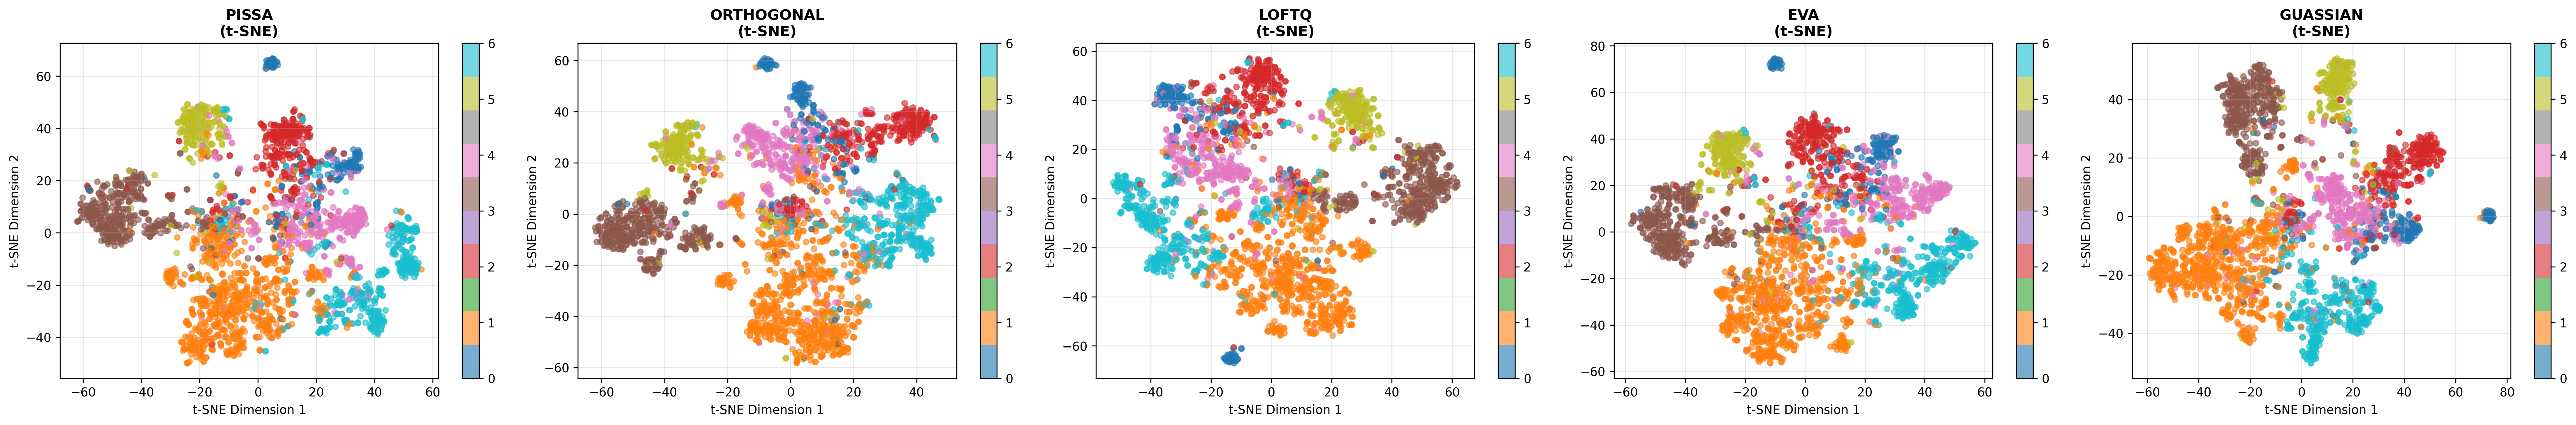
\includegraphics[width=\textwidth]{images/llama_3.2_1B_cora_lora_tsne_comparison.png}
	\caption{Overview of textual embeddings obtained from LLMs using different initial parameters.}
	\small
	Two-dimensional visualization of node embeddings using the t-SNE method for different versions of the language model trained on the Cora dataset. Differences in clustering patterns indicate the effect of parameter initialization on the semantic representations of nodes.
	\label{fig:tsne}
\end{figure}

As described in the proposed method, an LLM is fine-tuned on node text data specifically for the graph text classification task. Upon completion of the training process, node-level representations are extracted by applying a mean pooling operator over the textual representations associated with each node.

To qualitatively compare these representations, the node embeddings generated by each model version were mapped into a two-dimensional space using the t-SNE method  \citep{cai2022tsne}, the results of which are shown in Figure \ref{fig:tsne}. As evident from the plots, each trained language model, despite using identical data and labels, has achieved distinct spatial patterns and node clusterings. These variations demonstrate that changes in the initialization of trainable parameters can lead to distinct semantic interpretations of node texts, consequently producing diverse node-level representations.

\paragraph{Comparison of CKA metric for Embedding}
\paragraph{Prediction Disagreement Diffirent Embedding Set for GNN}

% adding result of cka 
% prediction disagreement for gnn

\subsection{Performance Comparison of Trainable Ensemble Learning vs. Simple Averaging}

\begin{table*}[t]
\centering
\caption{Comparison of ensemble learning performance using trainable weights versus simple averaging (Uniform).}
\label{tab:ensemble_results}

\begin{tabular*}{\textwidth}{@{\extracolsep{\fill}} lcccc @{}}
\toprule
\multirow{2}{*}{\textbf{Dataset}} & \multirow{2}{*}{\textbf{Method}} 
& \multicolumn{3}{c}{\textbf{Performance Metrics}} \\
\cmidrule(lr){3-5}
 &  & \textbf{Accuracy} & \textbf{Macro-F1} & \textbf{Weighted-F1} \\
\midrule

\multirow{4}{*}{PubMed}
& Uniform    & 96.25 & 95.73 & 96.24 \\
& Ensemble1  & 96.98 & 96.56 & 96.97 \\
& Ensemble2  & 97.13 & 96.74 & 97.13 \\
& Ensemble3  & \textbf{97.16} & \textbf{96.75} & \textbf{97.16} \\
\midrule

\multirow{4}{*}{CiteSeer}
& Uniform    & 80.41 & 77.41 & 80.09 \\
& Ensemble1  & 81.66 & \textbf{79.25} & 81.50 \\
& Ensemble2  & 81.97 & 78.83 & 81.51 \\
& Ensemble3  & \textbf{82.13} & 79.04 & \textbf{81.61} \\
\midrule

\multirow{4}{*}{WikiCS}
& Uniform    & 87.74 & 86.44 & 87.78 \\
& Ensemble1  & 88.34 & 86.96 & 88.35 \\
& Ensemble2  & 88.38 & 87.03 & 88.40 \\
& Ensemble3  & \textbf{88.42} & \textbf{87.18} & \textbf{88.43} \\
\midrule

\multirow{4}{*}{Cora}
& Uniform    & 92.07 & 90.55 & 92.12 \\
& Ensemble1  & 93.17 & \textbf{92.06} & 93.14 \\
& Ensemble2  & \textbf{93.36} & 91.80 & \textbf{93.32} \\
& Ensemble3  & 93.17 & 91.85 & 93.14 \\
\midrule

\multirow{4}{*}{ArXiv}
& Uniform    & 77.69 & 63.77 & 77.07 \\
& Ensemble1  & \textbf{77.89} & \textbf{63.88} & \textbf{77.26} \\
& Ensemble2  & 77.76 & 63.16 & 77.07 \\
& Ensemble3  & 77.81 & 63.52 & 77.18 \\
\bottomrule
\end{tabular*}
\end{table*}

In Table \ref{tab:ensemble_results}, the performance of the three proposed trainable ensemble learning methods is compared with the simple averaging-based ensemble approach (Uniform) across the aforementioned datasets using three evaluation metrics. Based on the obtained results, all three proposed trainable methods deliver superior performance compared to the simple averaging approach.

Furthermore, according to the results in the table, the third proposed trainable ensemble method achieves the best overall performance across the majority of the datasets compared to the other two proposed versions.

\subsection{DIVERGE on Diffirent Encoder}


\subsection{ABLATION Study}
\subsubsection{Error Rate Comparison: Ensemble Learning vs. GNNs}

\begin{figure}
    \centering
    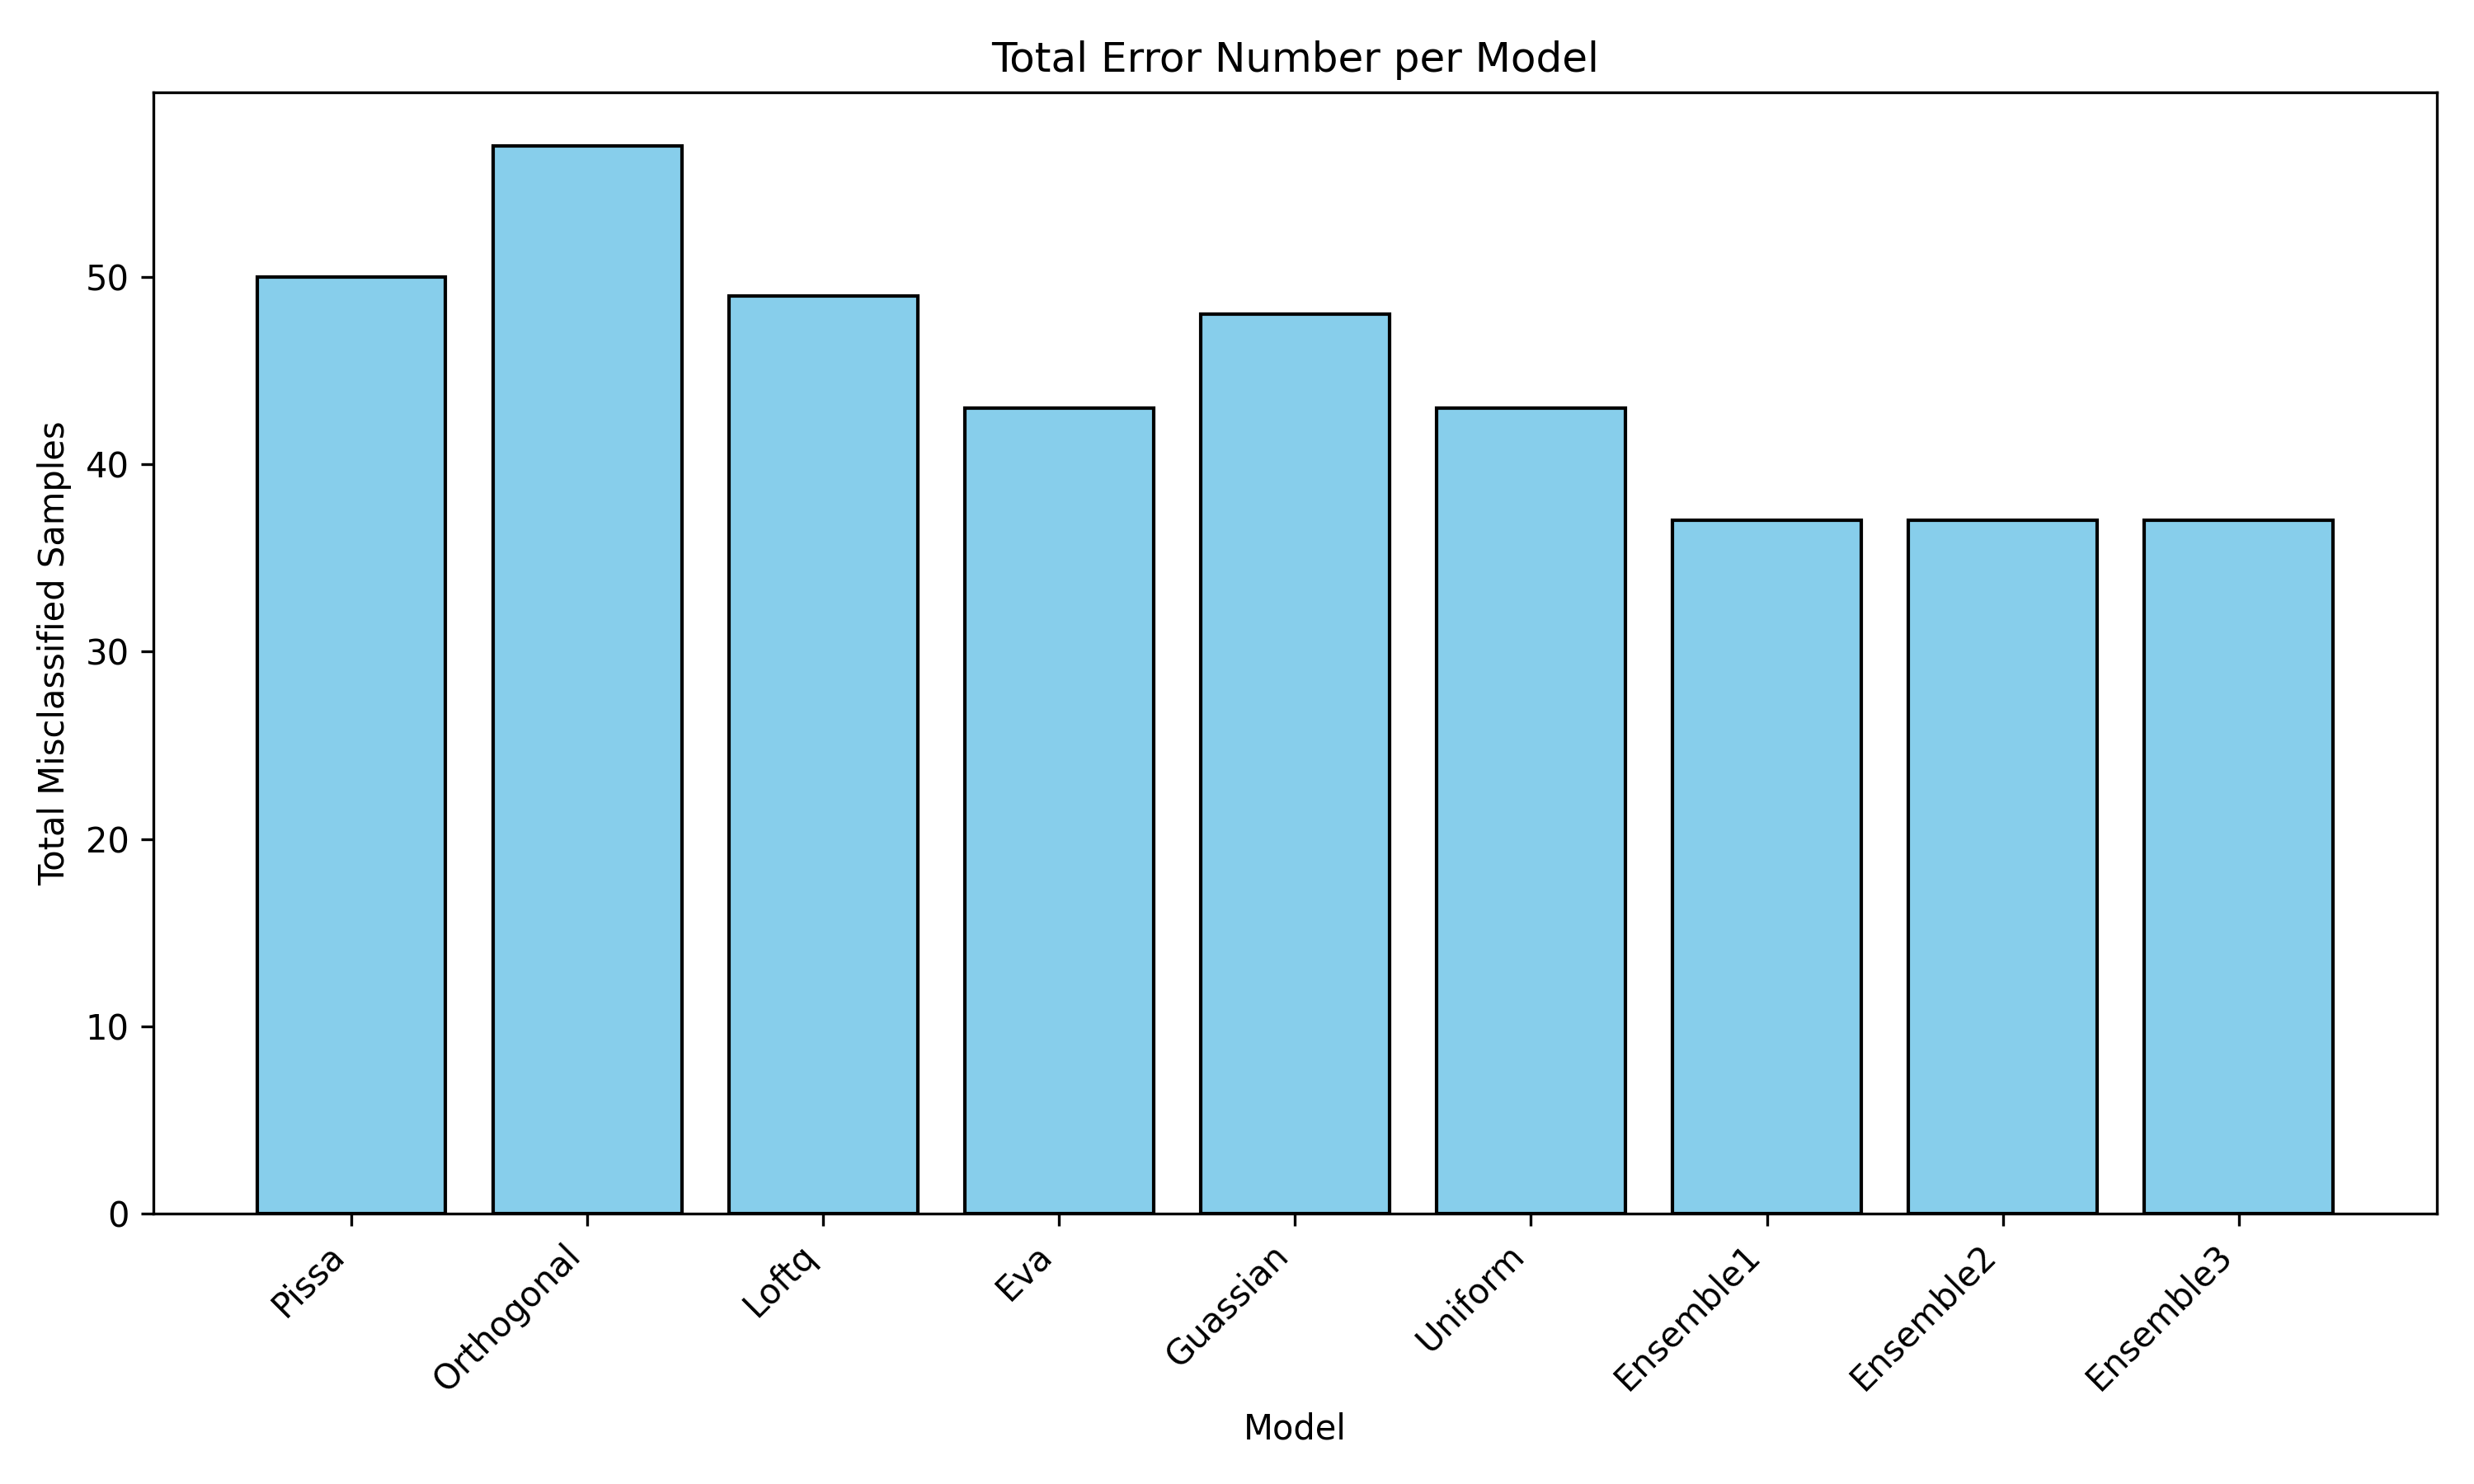
\includegraphics[scale=0.6]{images/gnn_total_error_numbers.png}
    \caption{Comparison of the total number of classification errors between individual models and ensemble learning methods.}
    \small
    The reduction in the number of errors in ensemble methods demonstrates the effective utilization of the diversity in textual representations derived from different initializations.
    \label{fig:error_numbers}
\end{figure}

\begin{table}[ht]
\centering
\caption{Comparison of error rates per class for the Cora dataset.}
\label{tab:error_rates}

\begin{tabular*}{\textwidth}{@{\extracolsep{\fill}} lccccccc @{}}
\toprule
\multirow{2}{*}{\textbf{Model}} & \multicolumn{7}{c}{\textbf{Error Rate per Class (\%)}} \\
\cmidrule(lr){2-8}
 & \textbf{Class 0} & \textbf{Class 1} & \textbf{Class 2} & \textbf{Class 3} & \textbf{Class 4} & \textbf{Class 5} & \textbf{Class 6} \\
\midrule

PiSSA      & 44.44 & 2.58 & \textbf{2.78} & 1.20 & 22.39 & 7.89 & 9.89 \\
Orthogonal & 38.89 & 2.58 & 18.06 & 2.41 & 13.43 & 7.89 & 13.19 \\
LoFTQ      & 33.33 & 2.58 & 8.33 & 1.20 & 16.42 & 7.89 & 13.19 \\
EVA        & 25.00 & \textbf{1.29} & 8.33 & 1.20 & 16.42 & 7.89 & 12.09 \\
Gaussian   & 22.22 & 2.58 & 15.28 & 2.41 & 11.94 & 7.89 & 13.19 \\
\midrule
Uniform    & \textbf{13.89} & 3.87 & 12.50 & 1.20 & \textbf{13.43} & 7.89 & 10.99 \\
\midrule
Ensemble1  & \textbf{13.89} & \textbf{1.94} & 8.33 & 1.20 & 16.42 & \textbf{7.89} & \textbf{8.79} \\
Ensemble2  & 19.44 & 2.58 & \textbf{6.94} & \textbf{0.00} & 14.93 & \textbf{7.89} & \textbf{8.79} \\
Ensemble3  & 19.44 & 2.58 & \textbf{6.94} & 1.20 & \textbf{13.43} & \textbf{7.89} & \textbf{8.79} \\
\bottomrule
\end{tabular*}
\end{table}


Table \ref{tab:error_rates} illustrates the error rate for each class, and Figure \ref{fig:error_numbers} presents the total number of classification errors for various models. The individual models consist of GNNs trained using embeddings from different initialization strategies. Additionally, the performance of the ensemble learning method in simple averaging mode (Uniform) and the three proposed trainable versions is reported.

Analysis of the results indicates that the trainable ensemble learning methods achieve the lowest or second-lowest error rates in most classes. This suggests that the proposed ensemble framework is capable of effectively combining the complementary information present in the individual models. 

Furthermore, it is observed that the proposed trainable ensemble methods outperform simple averaging in the majority of classes. This indicates that learning the combination coefficients in a data-driven manner can yield better performance compared to a static and uniform aggregation of models.




\subsubsection{Analysis of the Impact of Fine-Tuning on the Quality of Textual Embeddings}

The objective of this experiment is to investigate whether fine-tuning a LLM can yield a statistically significant improvement in downstream performance. To this end, textual embeddings of the graph are extracted in two states: 
(1) prior to fine-tuning and 
(2) after fine-tuning.

Subsequently, a separate GNN is trained using each set of embeddings. Finally, the two resulting models are evaluated on the same samples in the test set, and their results are compared pairwise.

Since both models are evaluated on identical samples and their outputs are recorded as correct/incorrect for each sample, \textbf{McNemar's Test} is employed for the statistical comparison. This test is suitable for comparing two dependent classifiers.

The statistical hypotheses are defined as follows:
\[
H_0: \text{The error rates of the fine-tuned model and the base model are equal.}
\]
\[
H_1: \text{There is a significant difference between the error rates of the two models.}
\]

The McNemar test statistic is defined as:
\begin{equation}
\chi^2 = \frac{(b - c)^2}{b + c}
\end{equation}

where:
\(b\) is the number of samples correctly classified by the base model but incorrectly by the fine-tuned model,  
and \(c\) is the number of samples correctly classified by the fine-tuned model but incorrectly by the base model.

In this research, the significance level is set at \(\alpha = 0.05\).

The results of McNemar's test for various datasets are presented in Table \ref{tab:mcnemar}.

\begin{table}[h]
\caption{Results of McNemar's test comparing the performance of GNNs based on embeddings extracted before and after LLM fine-tuning. The values $b$ and $c$ represent discordant pairs, from which the test statistic and $p$-value are calculated.}
\label{tab:mcnemar}

\begin{tabular*}{\textwidth}{@{\extracolsep{\fill}} lcccc @{}}
\toprule
\textbf{Metric} & \textbf{Cora} & \textbf{PubMed} & \textbf{CiteSeer} & \textbf{WikiCS} \\
\midrule
Both Correct & 433 & 3538 & 533 & 1955 \\
Base Model Only Correct ($b$) & 11 & 40 & 10 & 70 \\
Finetuned Only Correct ($c$) & 64 & 267 & 38 & 102 \\
Both Wrong & 34 & 99 & 57 & 214 \\
Discordant Pairs ($b+c$) & 75 & 307 & 48 & 172 \\
McNemar Statistic & $36.053$ & $166.371$ & $15.188$ & $5.587$ \\
$p$-value & $1.92\times10^{-9}$ & $4.59\times10^{-38}$ & $9.73\times10^{-5}$ & $0.0181$ \\
\midrule
\textbf{Result} & Reject $H_0$ & Reject $H_0$ & Reject $H_0$ & Reject $H_0$ \\
\bottomrule
\end{tabular*}
\end{table}

Based on the results in Table \ref{tab:mcnemar}, the $p$-value for all datasets was less than the significance level \(\alpha = 0.05\); therefore, the null hypothesis is rejected in all cases. These findings indicate that fine-tuning the LLM has led to a statistically significant improvement in the downstream performance of the GNN.

\subsubsection{Analysis of the Impact of Number of Finetuned LLM}
% in this section we analysie the impact of parameter of M

\subsubsection{Computation Efficiency with Parralisim}

\subsubsection{Comparision of Ensemble Methods}

\section{Discussion}\label{sec:Discussion}

This section interprets the experimental evidence, states the theoretical and practical implications of DIVERGE, and clarifies how the proposed framework differs from representative prior TAG methods summarized in Table~\ref{tab:related_gap}.

\subsection{Interpretation of main findings}\label{sec:resultsAnalysis}

The results in Tables~\ref{tab:diverge_node_classification_accuracy_sota} and~\ref{tab:diverge_node_classification_macro_f1_sota} support a single overarching claim: \emph{representation diversity induced by LoRA initialization, rather than textual augmentation, is sufficient to outperform augmentation-heavy LLM--GNN pipelines when node texts are already informative}. On all five benchmarks, DIVERGE achieves the best reported accuracy and Macro-F1 among compared methods, including classical GNNs, frozen- and fine-tuned-language-model encoders, and hybrid approaches such as TAPE, ENGINE, and LLaGA. Relative to the strongest augmentation-based baseline (TAPE), DIVERGE improves accuracy by 1.31--5.68 percentage points across datasets, with the largest gains on Cora and CiteSeer, where topic boundaries are fine-grained and class imbalance is more pronounced.

Three mechanisms explain these improvements. First, different LoRA initialization strategies produce semantically distinct node embeddings despite identical training texts and labels, as evidenced by the t-SNE visualizations in Figure~\ref{fig:tsne} and the heterogeneous per-class error profiles in Table~\ref{tab:error_rates}. Each initialization captures a complementary semantic view of the same nodes, so the resulting GNN pool is genuinely diverse rather than redundant. Second, trainable ensemble learning exploits this diversity more effectively than uniform averaging: all three proposed aggregation schemes outperform the Uniform baseline (Table~\ref{tab:ensemble_results}), and class-level weighting reduces errors on minority classes that individual GNNs misclassify. Third, LLM fine-tuning itself yields statistically significant downstream gains, as confirmed by McNemar's test on four datasets (Table~\ref{tab:mcnemar}), indicating that the encoder stage materially improves GNN inputs rather than merely recombining fixed representations.

Together, these findings answer the motivating question posed in Section~\ref{sec:Preliminaries}: competitive performance \emph{can} be achieved without textual augmentation when diversity is induced directly from native node texts through multiple parameter-efficient fine-tuning trajectories and adaptively ensembled GNN predictions.

\subsection{Theoretical implications}

From a theoretical standpoint, DIVERGE advances TAG research in three ways.

\textbf{Diversity from optimization trajectories.} Most LLM--GNN pipelines derive diversity from different \emph{modalities} or pipeline stages---for example, augmented versus native text (TAPE), retrieved versus local context (SKETCH), or task-adaptive prompting (LLM-BP). DIVERGE instead treats \textbf{LoRA initialization diversity} as a controllable source of complementary semantic subspaces for the same backbone encoder. This extends parameter-efficient fine-tuning theory \citep{Hu2021LoRA, meng2024pissa, paischer2024eva} to graph learning and shows that multiple low-rank adaptation trajectories can explore distinct local minima even under identical node texts and labels.

\textbf{Limits of textual augmentation.} The preliminaries in Section~\ref{sec:Preliminaries} and the Cora feature comparison in Table~\ref{tab:gnn_features_comparison} demonstrate that LLM-generated augmentations can \emph{degrade} performance when native texts are already rich. DIVERGE provides empirical confirmation at scale: it surpasses TAPE on all five benchmarks without generating explanations, summaries, or pseudo-labels. Theoretically, this suggests that augmentation should be treated as a conditional strategy---beneficial when texts are sparse or noisy, but potentially harmful when native semantics are sufficient---rather than as a default prerequisite for LLM--GNN integration.

\textbf{Adaptive aggregation over heterogeneous learners.} Uniform logit averaging assumes equal utility across models and classes, an assumption violated when different initializations specialize on different label groups (Table~\ref{tab:error_rates}). DIVERGE's learned model- and class-level weights formalize a more flexible fusion principle: ensemble coefficients should be data-dependent and class-aware. This aligns with broader ensemble-learning theory while offering a concrete, trainable alternative to fixed averaging in TAG pipelines.

Finally, the results corroborate the LLMNodeBed finding that strong \emph{local} encoders are often more reliable than costly enhancers \citep{Wu2025LLMNode}. DIVERGE operationalizes this insight by investing compute in diverse encoder trajectories rather than in external API-based text generation.

\subsection{Positioning relative to prior work}

Table~\ref{tab:related_gap} summarizes the design differences; here we connect those differences to the empirical outcomes reported in Section~\ref{sec:Results}.

\textbf{Versus TAPE} \citep{he2024harnessing}: TAPE enriches node text via LLM explanations and zero-shot predictions, then uniformly averages multiple GNNs. DIVERGE uses native text only, induces diversity through multi-initialization LoRA, and learns ensemble weights. DIVERGE outperforms TAPE on every benchmark despite omitting augmentation and API calls, supporting the claim that initialization-driven diversity can substitute for generated text when node descriptions are informative.


\textbf{Versus UltraTAG} \citep{yu2025ultratag}: UltraTAG modularizes augmentation, encoding, and training into a configurable pipeline that may still rely on optional external services. DIVERGE offers a narrower but more deployable encoder--ensemble design with a single diversity mechanism (LoRA initialization) and no augmentation module, achieving stronger results on the LLMNodeBed benchmarks used here.

\textbf{Versus LLM-BP} \citep{wang2025llmbp}: LLM-BP introduces diversity through task-adaptive prompting and fuses information via belief propagation on a single embedding space. DIVERGE derives diversity from multiple fine-tuning trajectories of one backbone and fuses GNN logits through learned ensemble weights. The two approaches are complementary in philosophy---graph-adaptive propagation versus heterogeneous-model ensembling---and DIVERGE's gains on the shared benchmarks suggest that multi-trajectory encoding merits equal consideration alongside task-adaptive single encoders.

\textbf{Versus SKETCH} \citep{zhou-etal-2025sketch}: SKETCH retrieves related texts and distant structural contexts to enrich LM inputs and reduces reliance on conventional GNN propagation. DIVERGE stays GNN-centric and uses only each node's native text, offering a complementary design point: diversity from encoder initialization rather than from retrieved cross-node context. Both methods avoid paid API augmentation, but DIVERGE targets settings where local node text is informative and graph propagation through GNNs remains desirable.

\textbf{Versus STAGE} \citep{zolnai-lucas-etal-2024-stage}: STAGE ensembles GNNs trained on embeddings from a \emph{single} frozen LLM. DIVERGE goes further by generating multiple adapted encoders through LoRA and learning non-uniform combination weights, explaining its consistent accuracy and Macro-F1 advantages.

In summary, no prior TAG method simultaneously (i)~induces representation diversity through multi-initialization LoRA on native node text, (ii)~trains a pool of GNNs on complementary embeddings, and (iii)~fuses predictions with learned model- and class-level weights---all without textual augmentation or external APIs. DIVERGE fills this gap empirically on five standard benchmarks and conceptually by reframing diversity as an encoder-side, initialization-driven property rather than an augmentation-side artifact.


\section{Limitations}\label{sec:Limitations}

Despite the strong performance of the proposed DIVERGE framework, several limitations remain.

First, the proposed method demonstrates stronger performance in fully supervised settings compared to semi-supervised scenarios. The primary reason is that the adaptive ensemble learning framework relies on sufficient labeled data in order to effectively learn the contribution and weighting of different models. In semi-supervised settings, where only a limited number of labeled nodes are available, the ensemble model may not accurately estimate the optimal combination coefficients, which can reduce the overall effectiveness of the framework.

Second, although the proposed approach eliminates the need for costly textual augmentation and external LLM API calls, it does not fully exploit all capabilities of LLMs. In this work, LLMs are mainly utilized as semantic encoders for extracting node-level textual representations. However, recent studies have shown that LLMs can also play important roles as graph enhancers, for example through structural refinement, semantic edge generation, textual augmentation, or label enhancement. These capabilities were not extensively explored in the current framework.

Another limitation is the computational overhead associated with training multiple LLMs and GNNs using different initialization strategies. Although parameter-efficient fine-tuning methods such as LoRA significantly reduce the number of trainable parameters, the overall training process still requires multiple independent optimization stages and additional memory resources for storing several models simultaneously.

Finally, the proposed framework was mainly evaluated on citation-based text-attributed graphs containing relatively rich textual information. Therefore, the generalization ability of the method to graphs with short, noisy, or low-quality texts (such as social media graphs or recommendation systems) remains an open research question.

Future work can address these limitations by designing more robust ensemble mechanisms for low-label regimes, integrating structural and textual enhancement capabilities of LLMs, reducing the computational complexity of multi-model training, and extending the framework to broader categories of text-attributed graphs.

\section{Conclusion}\label{sec:Conclusion}

In this paper, we proposed \textbf{DIVERGE}, a novel framework for learning on text-attributed graphs that combines LLMs and GNNs through diverse representation learning and adaptive ensemble mechanisms. Unlike previous approaches that rely heavily on expensive textual augmentation or external LLM APIs, the proposed method demonstrates that diverse and complementary node representations can be effectively generated solely from the original graph texts by utilizing multiple LoRA fine-tuning strategies with different parameter initializations.

To achieve this objective, multiple parameter-efficient LLMs were independently fine-tuned using different initialization methods, and the extracted textual representations were used to train multiple GNNs. Subsequently, an adaptive ensemble learning framework was introduced to combine the outputs of these graph models through trainable weighting mechanisms at both the model and class levels. Experimental results on several benchmark text-attributed graph datasets, including Cora, CiteSeer, PubMed, WikiCS, and OGBN-ArXiv, demonstrated that the proposed framework consistently outperforms existing GNN-based and hybrid LLM-GNN baselines in terms of Accuracy and Macro-F1 metrics.

Furthermore, the experimental analysis showed that different LoRA initialization strategies produce semantically distinct and complementary embeddings. The obtained results also confirmed that trainable ensemble learning methods provide superior performance compared to simple averaging strategies by more effectively exploiting the diversity among representations. In addition, statistical analysis using McNemar's test demonstrated that fine-tuning the LLM leads to statistically significant improvements in downstream graph learning performance.

Overall, the findings of this research suggest that representation diversity itself can serve as an effective alternative to costly textual augmentation for improving learning on text-attributed graphs. By relying on locally fine-tuned encoders rather than external LLM APIs, DIVERGE also offers a privacy-preserving deployment path for graphs whose node text cannot leave organizational or regulatory boundaries. The proposed framework opens new directions for integrating parameter-efficient LLM fine-tuning, representation diversity, and adaptive ensemble learning in graph-based machine learning systems.



%\printcredits


\section*{Data availability}
Benchmark datasets are available via \citep{Wu2025} (accessed 6 June 2026).
Source code for DIVERGE is publicly available at \url{https://github.com/nimaiparifard/DIVERGE}.
% [dataset] Wu, X. (2025). LLMNodeBed. Hugging Face Datasets. \url{https://huggingface.co/datasets/xxwu/LLMNodeBed/tree/main} (Accessed 6 June 2026).
% \end{thebibliography}

%% Loading bibliography style file
%\bibliographystyle{model1-num-names}
\FloatBarrier

\bibliographystyle{cas-model2-names}

% Loading bibliography database
\bibliography{cas-refs}

\end{document}

